\documentclass{article}
\usepackage{graphicx}
\usepackage[margin=1.5cm]{geometry}
\usepackage{amsmath}

\begin{document}
\twocolumn

\title{Tuesday Warm Up, Unit 0: Foundations and Fundamentals}
\author{Prof. Jordan C. Hanson}
\maketitle

\section{Memory Bank}
\small
\begin{itemize}
\item \textbf{Homogeneous system:} Let $k$ be a constant, and let $s_{\rm in}(t)$ and $s_{\rm out}(t)$ be the input and output signals to a system $S$, respectively.  $S$ is \textit{homogeneous} if:
\begin{align}
s_{\rm out}(t) &= S[s_{\rm in}(t)] \\
k s_{\rm out}(t) &= S[k s_{\rm in}(t)]
\end{align}
\item \textbf{Additive system:} Let $s_{\rm 1}(t)$ and $s_{\rm 2}(t)$ be two input signals to a system $S$, with outputs $s'_{\rm 1}(t)$ and $s'_{\rm 2}(t)$.  $S$ is \textit{additive} if:
\begin{align}
s'_{\rm 1}(t) &= S[s_{\rm 1}(t)] \\
s'_{\rm 2}(t) &= S[s_{\rm 2}(t)] \\
s'_{\rm 1}(t)+s'_{\rm 2}(t) &= S[s_{\rm 1}(t)+s_{\rm 2}(t)]
\end{align}
\item \textbf{Shift-invariant system:} Let $s_{\rm in}(t)$ and $s_{\rm out}(t)$ be input and output signals to a system $S$, and let $t_0$ be a constant.  $S$ is \textit{shift invariant} if:
\begin{align}
s_{\rm out}(t) &= S[s_{\rm in}(t)] \\
s_{\rm out}(t-t_0) &= S[s_{\rm in}(t-t_0)] \\
\end{align}
\item \textbf{Synthesis:} combining input signal components together linearly to form an output signal.
\item \textbf{Decomposition:} producing the output signal components linearly from an input signal.
\item \textbf{Fundamental Concept of DSP:} Decomposing an input signal into components, passing them trough a linear system, and synthesizing the results produces the same output as passing the original signal through the system.
\item \textbf{Impulse signal:} a single nonzero point in a string of zeros.
\item \textbf{Impulse decomposition:} decomposing a digitized, sampled signal into a linear combination of impulse signals.
\item \textbf{Even/Odd decomposition:} decomposing a digitized, sampled signal into even and odd signal components.
\end{itemize}
\normalsize

\section{Linear Systems}

\begin{enumerate}
\item Let a system $S$ act on a signal $s(t)$ as follows: $S[s(t)] = s(t-T/2)$.  (a) If $s(t) = 2\sin(2\pi ft)$, and $T = 1/f$, what is $S[s(t)]$? (b) Graph the input and output of $S$. (c) What is $s(t) + S[s(t)]$? \\ \vspace{2cm}
\item Let a system $S$ act on a signal $s(t)$ as follows: $S[s(t)] = 2s - 1.5$. (a) If $s(t) = 1.5 \sin(2\pi(60)t)$, what is $S[s(t)]$? (b) If $s(t) = -1.5 \sin(2\pi(60)t)$, what is $S[s(t)]$? (c) Graph the outputs of (a) and (b). (d) Consider Fig. \ref{fig:1} (bottom).  Develop expressions for $y_1[n]$, $y_2[n]$, and $y_3[n]$, and show that each is linear. \\ \vspace{3cm}
\item Suppose a signal component is the impulse $x[n] = [0~0~0~2~0~0 ...]$, with 100 total samples.  (a) If $y[n] = S(x[n]) = -x[n-1]$, what is $y[n]$? (b) If $y[n] = S(x[n]) = (x[n])^2$, what is $y[n]$?  (c) Are the systems $S$ in parts (a) and (b) linear or non-linear? \\ \vspace{2cm}
\item Let $x[n]$ be a digitized, sampled signal with $N$ samples.  The \textit{even} component is $x_{\rm E} = (x[n] + x[N-n])/2$, and the \textit{odd} component is $x_{\rm O} = (x[n] - x[N-n])/2$. (a) Let $x[n] = [0~0~1~1~0~0]$.  Is it even or odd? (b) Let $x[n] = [0~-1~0~0~1~0]$.  Is it even or odd? 
\end{enumerate}

\begin{figure}
\centering
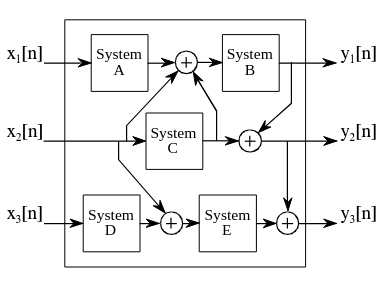
\includegraphics[width=0.33\textwidth]{commute_2.png}
\caption{\label{fig:1} A DSP system with multiple inputs and outputs.}
\end{figure}

\end{document}
